% Immutable scientific style asset from PR #19; v0.3 caption preserves transferred qualifications.
\begin{figure}[t]
\centering
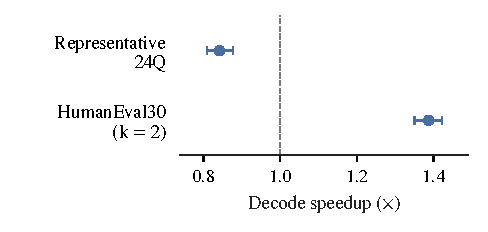
\includegraphics[width=\columnwidth]{../figures/style_v04/pdf/m4.pdf}
\caption{\textbf{Opposite profitability regimes on the same tested M4 stack}. Representative 24Q yields 0.842$\times$ [0.809, 0.877], while the separately preregistered HumanEval30 fixed-$k=2$ study yields 1.387$\times$ [1.351, 1.422]. Points are campaign prompt geometric means of paired decode speedups; intervals are campaign-specific 95\% prompt-bootstrap intervals. The dashed line marks parity. Both paths satisfy token equality (72/72 and 90/90 pairs), which is not functional HumanEval pass@$k$. These are separate studies, not a paired between-workload comparison; differing workloads and session conditions do not isolate workload-only causality.}
\label{fig:m4}
\end{figure}
